\documentclass[a4paper,11pt]{jsarticle} % ceostyを用いるための文書クラス

% 冊子形式にするには表紙(ページ数に含まれない)で
% 1ページ使っているので最後のページのページ番号が
% 4n  ->透かしがしにくい(表紙と裏表紙の裏面が白紙)
% 4n+1->一番微妙
% 4n+2->表紙と白紙の裏表紙ができる---こうなるように調整
% 4n+3->裏表紙も使う

\usepackage{fancyhdr}	% ページスタイル

%%スタイル
% 数式やテキストの描画
\usepackage{amsmath, amsfonts, amssymb, mathtools, mathrsfs, latexsym}	% ams関連は数式書くのに必須!!
%\DeclarePairedDelimiter{\abs}{\lvert}{\rvert}
\usepackage{nccmath, empheq}	% 結構ピンポイントなパッケージ

% 画像
%% 枠だけ表示(Cannot determine size of graphicと結構怒られる)
%\usepackage[draft]{graphicx}
%% 普通に表示させる(ただ重くなりやすい)
\usepackage[dvipdfmx]{graphicx}
\usepackage[dvipdfmx]{color}
\usepackage{here}	% 絶対Hereって勝手に呼んでるやつ
\usepackage{wrapfig}	% 回り込み(ceostyのymawarikomiもある)
\usepackage{subcaption}	% minipageを使って図を並べるときの各画像のキャプションに必要

% このファイルの肝.
% usepackageの順番(ceoとの前後関係)を変えると途端にエラーを吐くので注意
%\usepackage{ceo}
% 以下のパッケージはceostyの煽りをくらったもの
\usepackage{enumerate, comment}	% 順に文書モードでの段落環境, 複数行コメント

\pagestyle{fancy}
  \cfoot{\thepage}
  \renewcommand{\headrulewidth}{0pt}

\newcommand{\vevenspace}{\vspace{\stretch{1}}}	
\newcommand{\hruleline}{\par\noindent\hrulefill\par}
\newcommand{\length}[1]{$\overline{\textup{#1}}$}
\renewcommand{\eq}{$=$}
\newcommand{\vreidai}{\vspace{\stretch{0.3}}}
\newcommand{\nn}{$n$}
\newcommand{\m}{$m$}
\newcommand{\kmath}{$k$}
\renewcommand{\O}{\textup{O}}
\newcommand{\Pn}[2]{$\textup{#1}_{#2}$}
\newcommand{\mathPn}[2]{\textup{#1}_{#2}}
\renewcommand{\P}{\textup{P}}
\newcommand{\Q}{\textup{Q}}
\newcommand{\R}{\textup{R}}
\newcommand{\A}{\textup{A}}
\newcommand{\B}{\textup{B}}
\newcommand{\C}{\textup{C}}
\newcommand{\D}{\textup{D}}
\newcommand{\numseq}[2]{$\{#1_{#2}\}$}
\newcommand{\combi}[2]{{}_{#1}\mathrm{C}_{#2}}
\newcommand{\xy}{$xy$}
\newcommand{\yz}{$yz$}
\newcommand{\xz}{$xz$}
\newcommand{\zx}{$zx$}
\newcommand{\xyz}{$xyz$}
\newcommand{\x}{$x$}
\newcommand{\y}{$y$}
\newcommand{\z}{$z$}
\newcommand{\g}{$g$}


\newcounter{partNo}
\newcommand{\qPart}{
  \pagebreak
  \stepcounter{partNo}
  \noindent \textup{\Large 第\arabic{partNo}問} 
  \par \vspace{0.5\baselineskip}
}

\newcommand{\calcPage}{
  \pagebreak
  \begin{center}
    \textless\,計算用紙\,\textgreater
  \end{center}
  \pagebreak
}

\newcommand{\brankPage}{
  \pagebreak \mbox{} \pagebreak
}

%%%%%%%%%% メイン %%%%%%%%%%%
\begin{document}
%本文
\begin{titlepage}
  \begin{center}
    \vspace*{\stretch{1}}
    {\Huge\gt テスト演習}\\ \vspace{\baselineskip}
    \textup{\large 実施日:2023年10月21日}\\ \vspace{\stretch{1}}
  \end{center}
  \vfill
  \hfill {最終更新日:\today}
\end{titlepage}

\qPart
%!TEX root = *.tex
%%%%%%%%%%%%%%%%%%
% カウンタのリセット
% 問題文
滑車と糸の質量は無視できるものとし,重力加速度を\g とする.

\begin{enumerate}[〔A〕]
  \setlength{\leftskip}{-1.5zw}
  \setlength{\itemindent}{1zw}\setlength{\labelsep}{0.5zw}
  \setlength{\labelwidth}{1zw}\setlength{\leftmargin}{1zw}
  \setlength{\itemsep}{0.5\baselineskip}
  \item 図1のように,なめらかに回る定滑車に伸縮しない糸をかけて,糸の一方に質量$m_1$のおもりA,他方に質量$m_2$のおもりBをつけて静かに放した.
  \begin{enumerate}[(1)]
    \setlength{\leftskip}{-2.5zw}
    \setlength{\itemindent}{1zw}\setlength{\labelsep}{1zw}
    \setlength{\labelwidth}{1zw}
    \item $m_1 > m_2$のとき,おもりAが下降する加速度の大きさを求めよ.
    \item 糸に働く張力の大きさを求めよ.
    \item $m_1 + m_2 = \text{一定}$として,糸の張力を最大にする$m_1$と$m_2$の関係を求めよ.
  \end{enumerate}
  \item 次に,図2のように定滑車の一方に質量$3M$のおもりCを,他方に動滑車をつり下げて,動滑車には質量$2M$のおもりDと質量$M$のおもりEをつり下げた.C,D,Eを同時に静かに放した.
  \begin{enumerate}[(1)]
    \setlength{\leftskip}{-2.5zw}
    \setlength{\itemindent}{1zw}\setlength{\labelsep}{1zw}
    \setlength{\labelwidth}{1zw}
    \item おもりC,D,Eの加速度の大きさを求めよ.
    \item おもりD,E間の糸に働く張力の大きさを求めよ.
    \item おもりD,EはそのままでおもりCを$\C^\prime$に換えると,$\C^\prime$,D,Eを同時に静かに放しても,おもりは静止したまま動かなかった.
    このときのおもり$\C^\prime$の質量を求めよ.
  \end{enumerate}
\end{enumerate}

\begin{figure}[htbp]
  \centering
  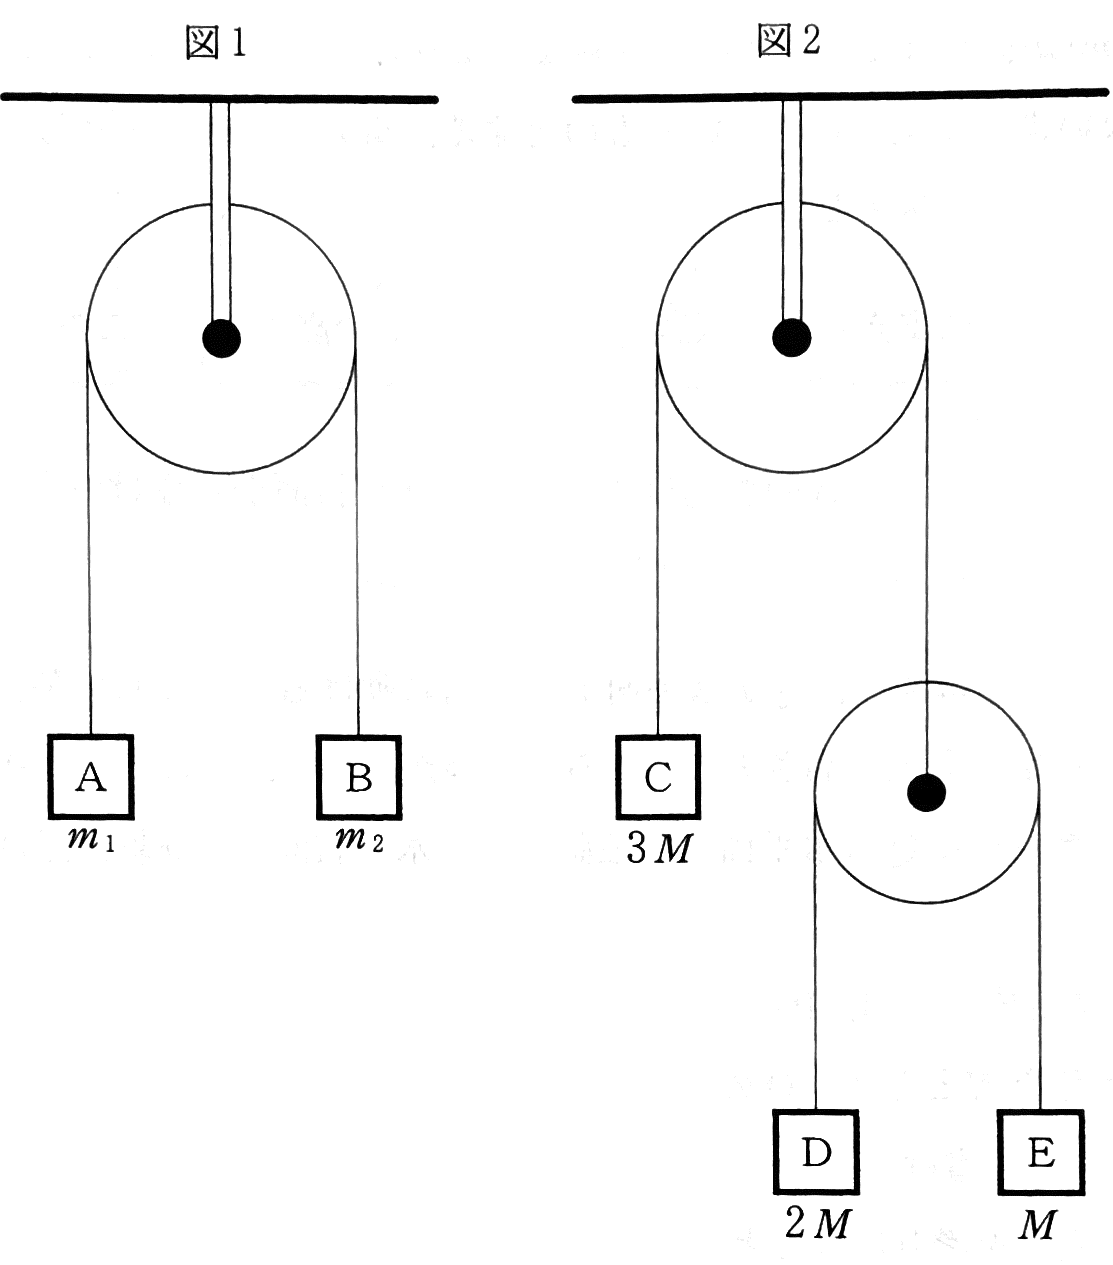
\includegraphics[width=20zw]{../graphs/se_1H_102.png}
\end{figure}


% メモ
\begin{comment}

\end{comment}


%%%%%%%%%%%%%%%%%%

\calcPage

\qPart
%!TEX root = *.tex
%%%%%%%%%%%%%%%%%%
% カウンタのリセット
% 問題文
{
\begin{wrapfigure}{r}{12zw}
  \vspace*{-\intextsep}
  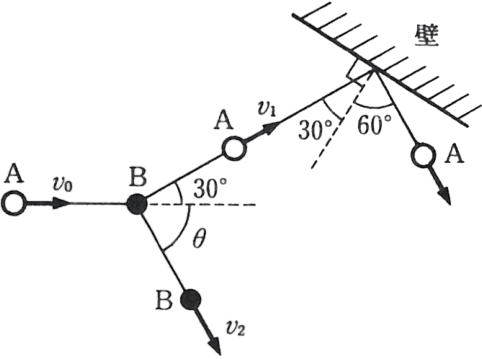
\includegraphics[width=12zw]{../graphs/se_1H_106.png}
\end{wrapfigure}
なめらかな水平面上に静止している小球Bに,質量$m$の小球Aが速さ$v_0$で衝突した.
衝突後の図のように,小球Aは進行方向に対し$30^\circ$の方向に進み,
小球Bは小球Aの衝突前の進行方向とゼロでない角$\theta$をなす方向に進んだ.
小球Aはその後水平面に垂直ななめらかな壁と,図のような角度で衝突してはね返った.
次の問いに答えよ.
\par}

\begin{enumerate}[(1)]
  \setlength{\leftskip}{-1.5zw}
  \setlength{\itemindent}{1zw}\setlength{\labelsep}{0.5zw}
  \setlength{\labelwidth}{1zw}\setlength{\leftmargin}{1zw}
  \item 小球AとBの衝突後の速さをそれぞれ$v_1,\,v_2$,またBの質量を$M$として,衝突における運動量保存則を,小球Aの衝突前の進行方向とそれに垂直な方向,それぞれの方向の成分について書け.
\end{enumerate}

衝突が弾性衝突であり,$v_1 = \dfrac{\sqrt{3}}{2}v_0$であることがわかったとする.
\begin{enumerate}[(1)]
  \setlength{\leftskip}{-1.5zw}
  \setlength{\itemindent}{1zw}\setlength{\labelsep}{0.5zw}
  \setlength{\labelwidth}{1zw}\setlength{\leftmargin}{1zw}
  \setcounter{enumi}{1}
  \item $v_0$と$m$を既知の量として,$v_0\,M,\,\theta$を求めよ.
  \item 衝突のとき小球AがBから受けた力積の大きさを求めよ.
  \item 衝突後,小球Bの得るエネルギーは,衝突前の小球Aの運動エネルギーの何倍か.
  \item 小球Aと壁との跳ね返り係数を求めよ.
  \item 小球Aが壁から受けた力積の大きさを求めよ.
  \item 小球Aが壁との衝突で失ったエネルギーを求めよ.
\end{enumerate}


% メモ
\begin{comment}

\end{comment}


%%%%%%%%%%%%%%%%%%

\calcPage

\brankPage

\brankPage

\brankPage

\end{document}